\documentclass[12pt]{Article}

% Package to handle graphics inclusion (optional)
\usepackage{graphicx}
% Package for better math formatting (optional)
\usepackage{amsmath}
% For references (optional)
\usepackage{cite}
% Package to customize title position
\usepackage{titling}
\usepackage{subcaption}
\usepackage{listings}
\usepackage{xcolor}
\usepackage{hyperref}

\lstset{
    language=Python,
    basicstyle=\ttfamily\small,
    keywordstyle=\color{blue},
    commentstyle=\color{gray},
    stringstyle=\color{red},
    showstringspaces=false,
    numbers=left,
    numberstyle=\tiny\color{gray},
    breaklines=true,
    frame=single,
    captionpos=b
}


\usepackage{silence}
\usepackage{wrapfig}
\usepackage{float}
\usepackage{adjustbox}
\usepackage[margin=0.8in]{geometry}  % Adjust the margin as needed

\setlength{\parindent}{15pt} 
% Adjust the title position
\setlength{\droptitle}{-6em}% Adjust the value as needed
% Title and Author information
\title{Lab 7 - Kubernetes Practice}
\author{
    Hugo Garrido-Lestache
}
\date{\today \\ CSC 5201 301}

\begin{document}

\maketitle
\section*{Introduction}
In this lab I will be using kubernetes to deploy a multi-pod application.
This application will be a simple falsk app which will connect to a sql datbase.
The flask app will have 3 pods and there will be 1 pod for the sql database.
\\
The sencond part of the lab I will be researching and describing an intresting use case for kubernetes.

\section{Kubernetes Practice}
After following the instructions in the lab I was able to deploy the application.
The application is a simple flask app that connects to a sql database.
once I deployed the app I was able to access the app from the browser.
Below is a screenshot of the app running in the browser in figure \ref{fig:app}.

\begin{figure}[H]
    \centering
    \fbox{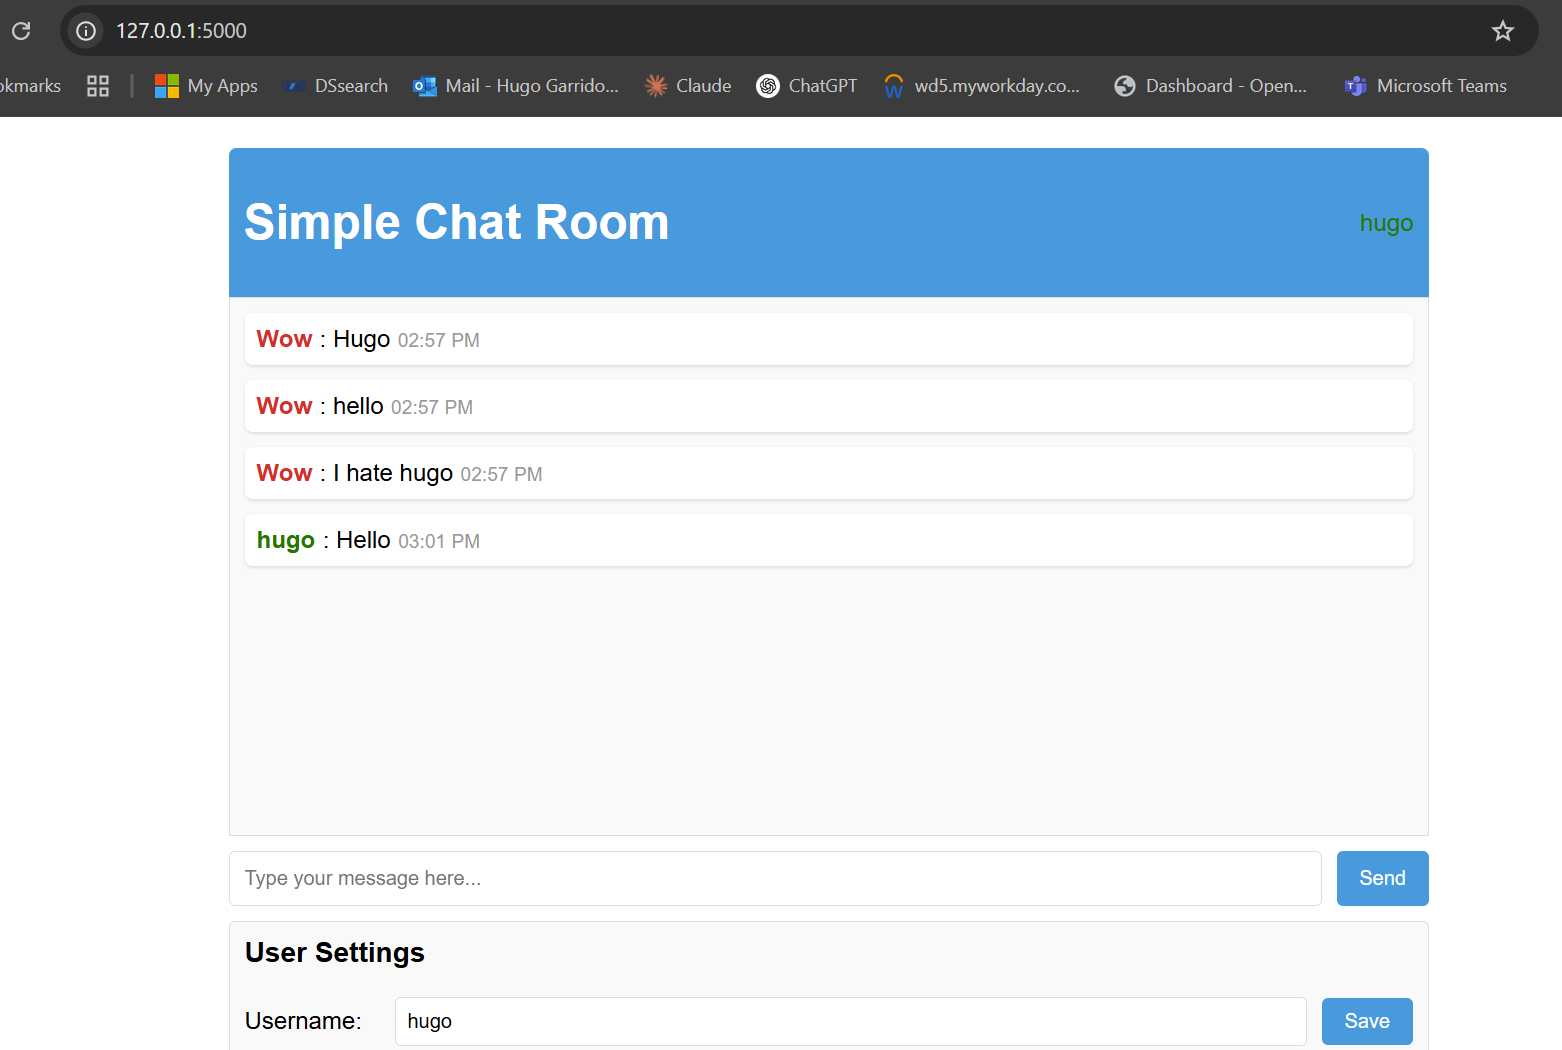
\includegraphics[width=0.8\textwidth]{images/1.png}}
    \caption{Flask app running in the browser}
    \label{fig:app}
\end{figure}

After ensuring the app was deployed I did curl request to the app to add a new user.
Below is me adding a new user to the database in figure \ref{fig:curl}.

\begin{figure}[H]
    \centering
    \fbox{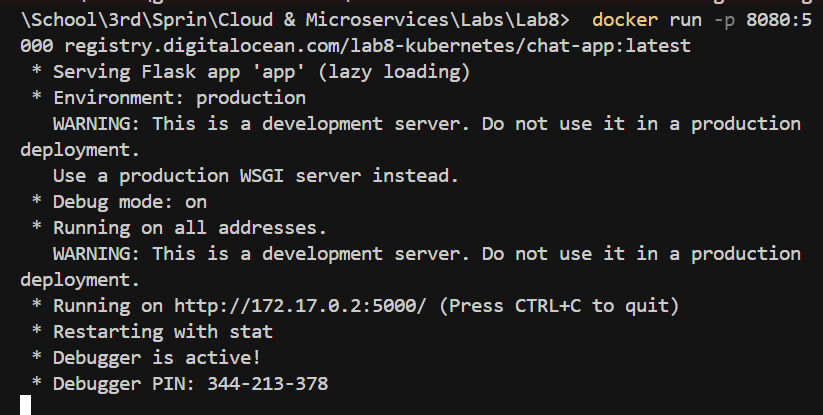
\includegraphics[width=0.8\textwidth]{images/2.png}}
    \caption{Curl request to add a new user to the database}
    \label{fig:curl}
\end{figure}

I then checked the database to ensure the user was added.
Below is a screenshot of the database with the new user in figure \ref{fig:db}.

\begin{figure}[H]
    \centering
    \fbox{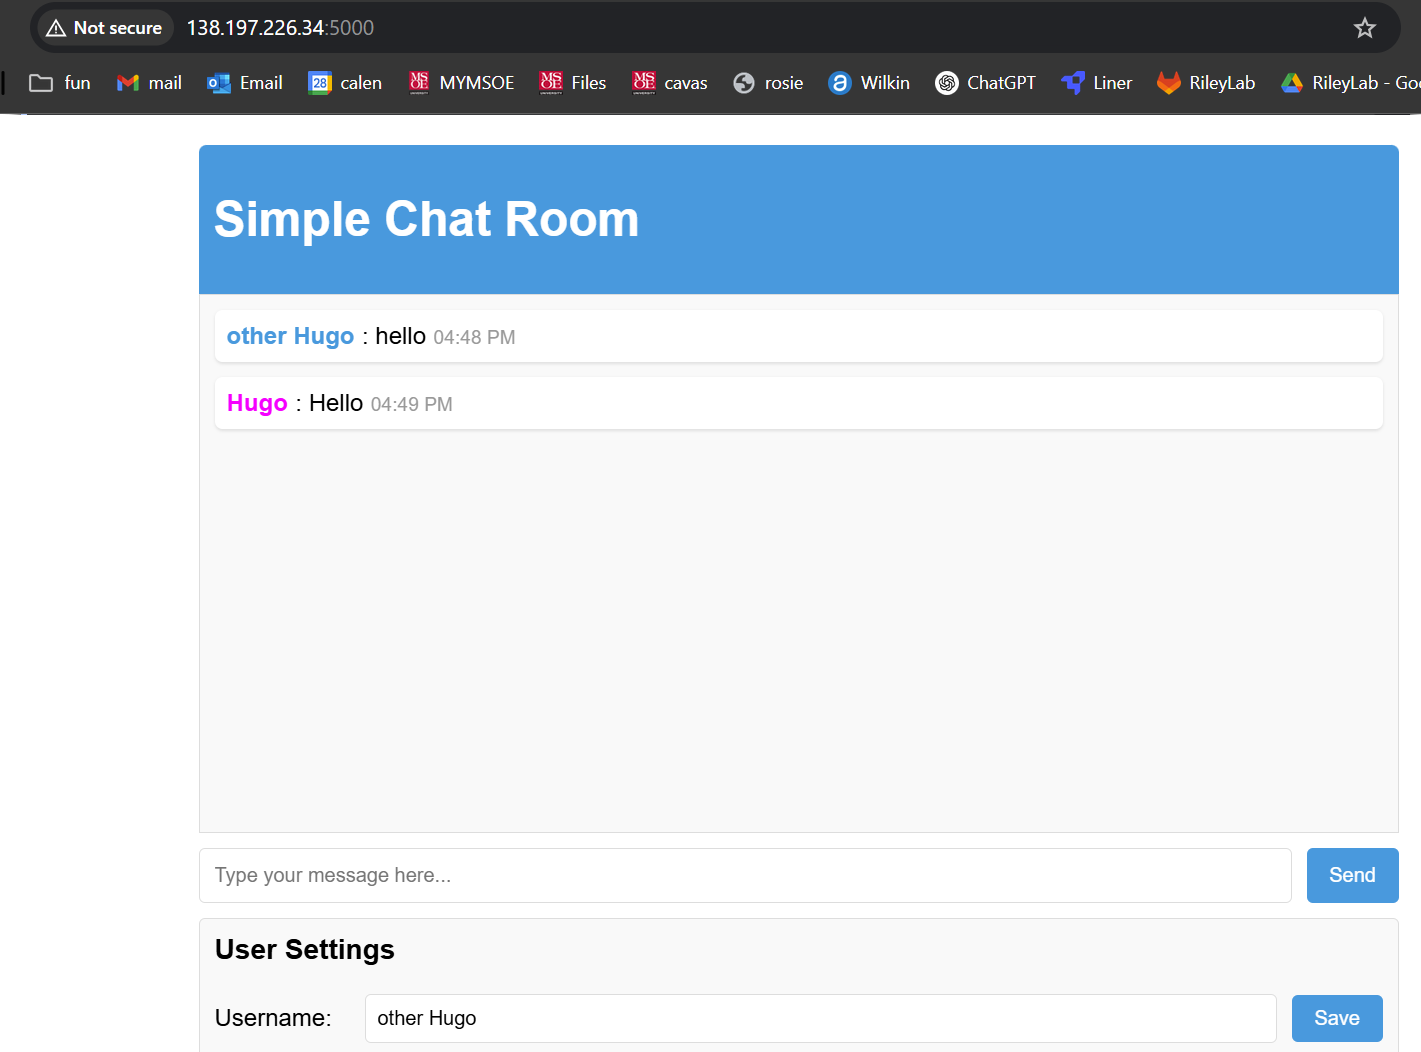
\includegraphics[width=0.8\textwidth]{images/3.png}}
    \caption{Database with the new user added}
    \label{fig:db}
\end{figure}

All these screenshot show that the application was deployed correctly and the database was connected to the flask app.
I also additionally checked the minikube dashboard to check on the status.
It was cool to see that there is a dashboard that shows the status of the pods and the services which is easy to acess and use.
Below is a screenshot of the minikube dashboard in figure \ref{fig:dashboard}.

\begin{figure}[H]
    \centering
    \fbox{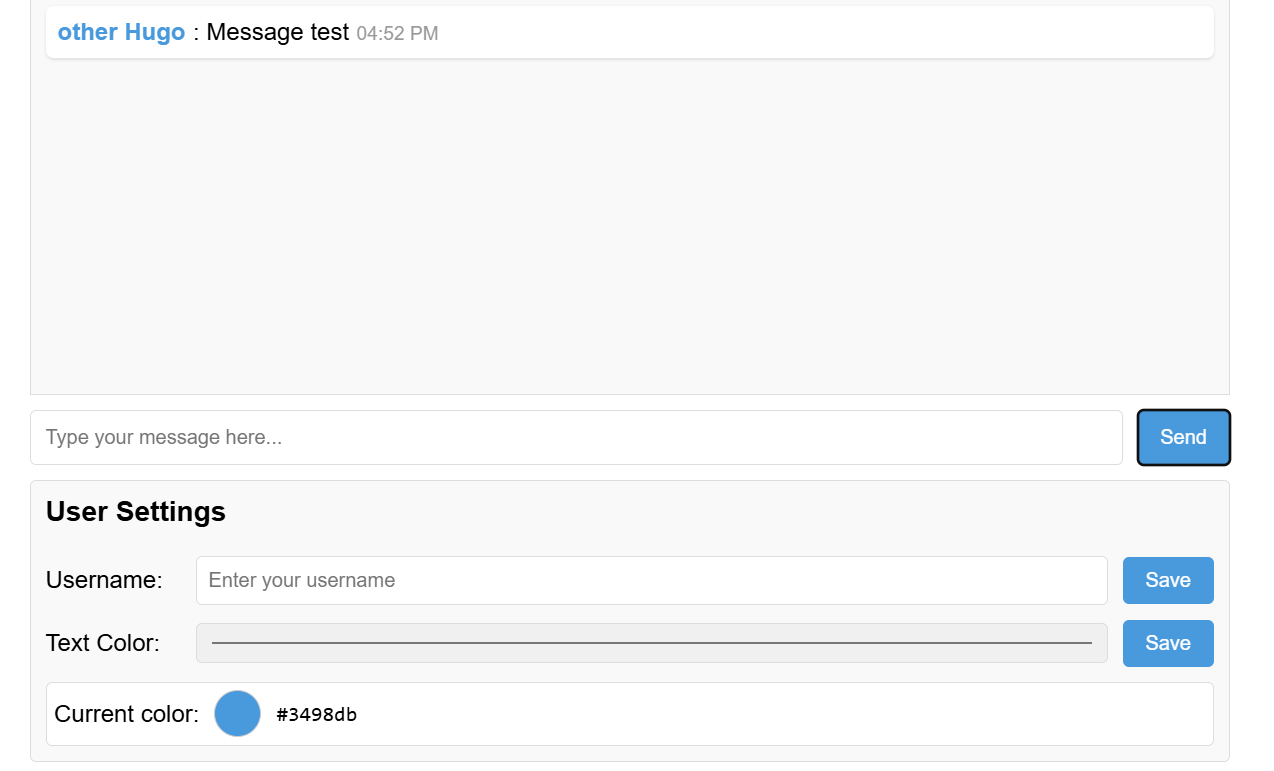
\includegraphics[width=0.8\textwidth]{images/4.png}}
    \caption{Minikube dashboard}
    \label{fig:dashboard}
\end{figure}

\clearpage
\section{Kubernetes Use Case}
The use case I am going to describe is going to be for training complex reinforcement learning models.
Reinforcement learning models difer from common machine learning models due to the fact that they dont just learn on data but also generate the data they learn from.
This is useally done in a loop where the collect data and then learn from that data repeatedly.
This process can be very computationally expensive and time consuming and could leverage from parallelization.
Additionally Reinforcement learning have a lot of hyperparameters that need to be tuned and this can also be done in parallel.
Additionally testing Reinforcement learning models may also be computationally expensive if the loss function is not directly tied to performance.

\subsection{How Kubernetes can help}
Kubernetes can help in many different ways and ideas.

\begin{enumerate}
  \item Faster training:
  By using Kubernetes we can speed up both the training through the data collections process by scaling up the number of pods which simulate the environment and collect data.

  \item Hyperparameter tuning:
  By using Kubernetes we can run multiple pods with different hyperparameters and then compare the results to see which hyperparameters work best.
  This can be done in quite intresting and complex methods such as terminating experiments early if they are not performing well and replacing them with new experiments.
  We can also allocate resources in a manner which is relative to the performance of the experiments allowing for more resources to be allocated to the better performing experiments.
  We can also be smart about how we select hyperparameters to try next by using bayesian optimization or other methods

  \item Testing simultanously:
  Some time measuring the quality of them model may also require some computational resources.
  Using kubernetes we could create a new pod when a model needs to be tested and then delete the pod once the test is done.
  This could allow for testing to be done in parallel and not slow down the training process.
\end{enumerate}

\subsection{Challenge with Pod networking}
Some potencial challenges that may arise may be the compunication between the pods.
Pods would have to communicate with with each other to share data and hyperparameters.
This could be done through a shared volume or through a shared database but this could be a potential bottleneck.

\subsection{Conclusion}
Kubernetes could be a very useful tool for training complex reinforcement learning models.
It could help speed up the final model training run time which may take days or weeks.
Allowing for automatic managing of testing and experimenting with hyperparameters.

Additionally if this is done in the cloud it gives you the ability to scale as much as you may want.
This could be useful as you could can use a lot of resources quickly rather than having to wait for a long time to get the resources you need.

\section*{feedback}
This Lab was quite intresting in understanding and actually getting experience with kubernetes and how it can be used.
I think I still need more undirected practive with kubernetes to better understand it but I think getting some initial experience was very helpful.
I has issues trying to deploy the app which boiled down to me not naming my python file correctly which was a bit frustrating but I was able to figure it out.
I think the lab was well structured and the instructions were clear and easy to follow.

The use case idea was good in getting us to understand the benefits of kubernetes and how it can be used in a real world scenario.
Thinking of you own usecase allows you to put your personal problems into perspective and see how kubernetes can help you solve them, making the lab more personal and intresting.
Overall I think the lab was very good and I learned a lot from it.



\end{document}
